\documentclass[10pt,a4paper]{article}

\usepackage[utf8]{inputenc}
\usepackage[spanish, activeacute]{babel}

\usepackage{graphicx} 

\usepackage{amsmath}
\usepackage{amsfonts}
\usepackage{amssymb}


\title{Principios y Métricas para el diseño de software}


\author{Pablo Echevarria - pablohe@gmail.com}
\date{Impreso: \today}

\begin{document}
\maketitle


\begin{description}
\item [Disclaimer ]
Documento sin ningún tipo de garantía ni 
revisión de la cátedra.
\item[Abstract] un un resumen de mis apuntes de clase 
y seguramente lleno de errores. 
Publicado en el sitio wiki del cuba.dc.uba.ar, con sus fuentes.
cualquier aporte y corrección será bienvenido.
Echo con latex y argouml. 
\end{description}

\newpage

\tableofcontents
\newpage
  
\section{Principios y Métricas}
\subsection{Herencia VS Delegación ó Metod Vs Strategy}

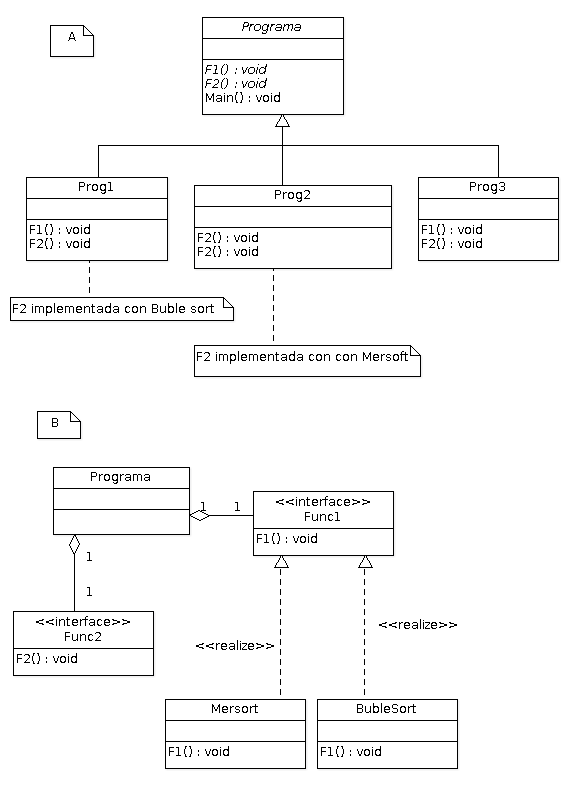
\includegraphics[scale=0.6]{./img/F1F2.png} 


En \textbf{a}, prog i no cambia dinámicamente, tengo que borrar la instancia y crear una nueva con
el método que me interesa ahora. ( mergsort por ej. )
En cambio en \textbf{b}, no. Esto sería un ejemplo de
\textit{Herencia VS Delegación ó Metod Vs Strategy }


Strategy, conviene cuando se que va a cambiar y/o cuando van a usarlo desde afuera.

\subsubsection{ Ejemplo: Ventana }
En \textbf{a} vemos como se podría resolver el problema: 
``una ventana como un rectángulo debe poder calcular su área''. Pero si en algún momento 
sale una versión de windows ``señor de los anillos edition'' y quiero una ventana circular fuimos!
Una mejor solución sería la propuesta en B.
Donde tengo en otro lado guardado el tipo de ventana y sin ni siquiera reiniciar la aplicación puedo cambiar el tipo de ventana.



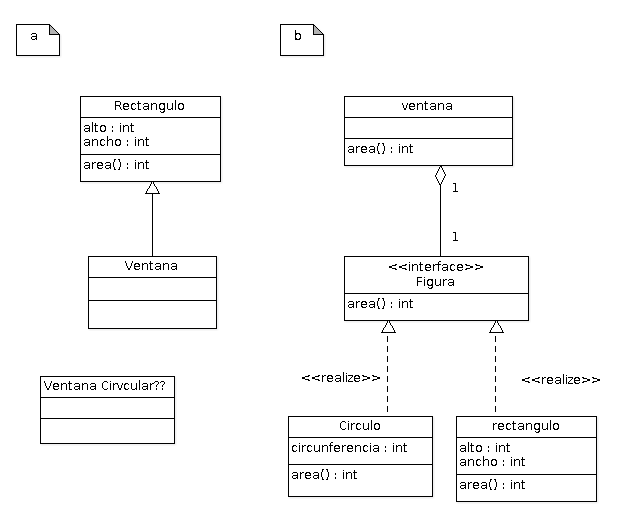
\includegraphics[scale=0.5]{./img/ventana-figura.png} 



\subsubsection{ Ejemplo:  Persona que camina }

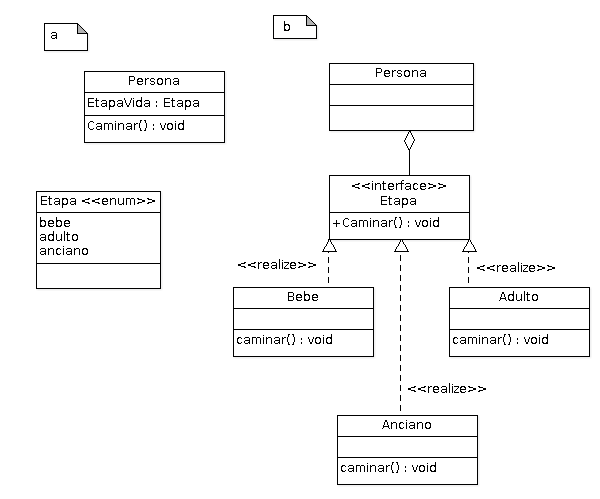
\includegraphics[scale=0.5]{./img/persona.png} 

Tenemos una persona que camina, pero no camina igual en todas las etapas de su vida,
la solución \textbf{a} parece estar bien, 
pero dentro de caminar debería preguntar en que etapa estoy 
y hacer lo que corresponda:
\begin{verbatim}
Caminar (){

  if(this.etapa == bebe)
      caminar en 4 patas

  if(this.etapa == adulto)
      caminar en 2 patas

  if(this.etapa == anciano)
      caminar en 3 patas
}
\end{verbatim}

No esta muy bueno ya que si hay una nueva etapa esta solución
no es extensible. 
En este caso es mejor depender de una abstracción, una persona tiene
una etapa ( una interfaz ) y la implemento con
un bebe, un adulto o un anciano. Si mañana hay uno nuevo
listo agrego el nuevo tipo que implementa la interfaz etapa y listo, esto se ve en \textbf{b}.


\subsection{Cohesión y Acoplamiento}

\subsubsection{Cohesión}
Correlación funcional entre los métodos en una entidad de software,
cada método hace una sola cosa, cada uno tiene una responsabilidad.

\subsubsection{Ejemplo: Aplicación gráfica}
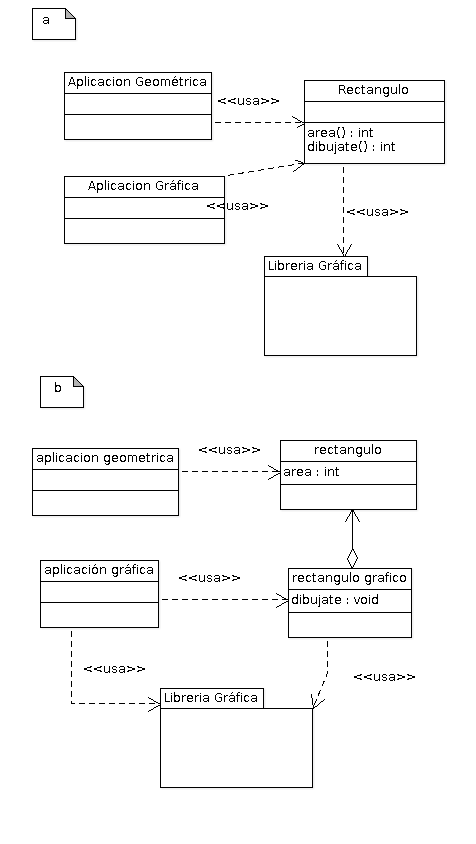
\includegraphics[scale=0.5]{./img/aplicacion-grafica-geometrica.png} 

En \textbf{a} vemos la clase rectángulo con sus 2 métodos, dibujate y calcular área.
La cuestión es que si cambio el rectángulo ( por que hago que se dibuje de otra forma, por ej.)
que tienen que ver eso con la aplicación geométrica  a la que solo le importa el calculo del área.
bueno no importa como hay un vinculo de usa debo re-testearla.
Una solución con menor cohesión sería la propuesta en \textbf{b}, ahora tenemos un  rectángulo que sabe calcular su área y un rectángulo gráfico ( que tienen un rectángulo) que sabe dibujarse.


 
\subsubsection{Ejemplo: Modem}
	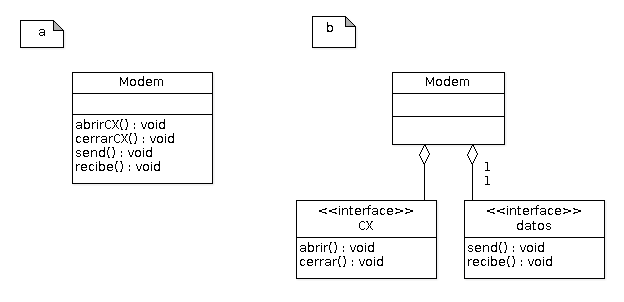
\includegraphics[scale=0.5]{./img/modem.png} 

	Tendríamos 2 funcionalidades claras, abrir y cerrar la cx 
	y por otro lado enviar y recibir datos.
	¿ Por que todo en la misma clase ? claramente hay 2 ejes de cambio.

\subsubsection{Acoplamiento}
en palabras de 2 letras: muchos <<usa>> en el diagrama de clases, 
el problema es que si alago cambia, debo re-testear todas las clases que la usan.


\section{Principios}

\subsection{SRP (Single Responsability Principle)}

\subsubsection{Ejemplo: Empleado persistidor }

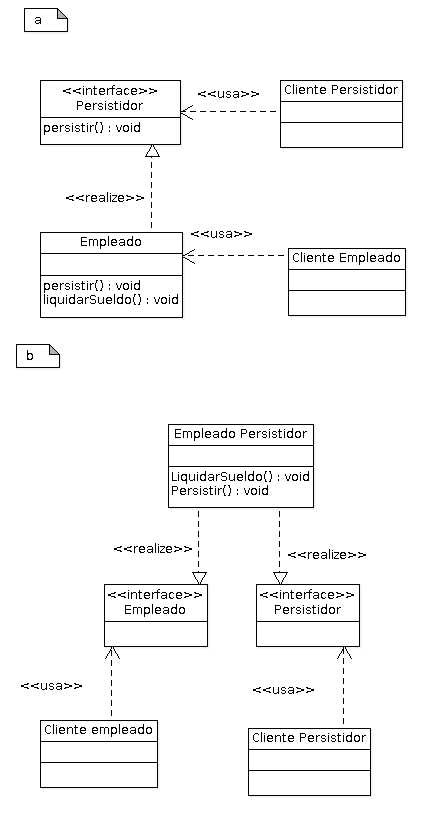
\includegraphics[scale=0.6]{./img/empleado-persistidor.png} 

En a tenemos la interfaz persistidor. Un empleado que tiene  un método, persistir y otro liquidar sueldo. Por otro lado alguien usa liquidar sueldo del empleado, 
no estaría bueno hay 2 razones de cambio para empleado, podremos separarlo con 2 interfaces, como en \textbf{b}.


\subsection{DIP (Dependency Inversion Principle)}
Cambie las direcciones de las flechas $<<$usa$>>$

\subsubsection{Ejemplo: Estufa }
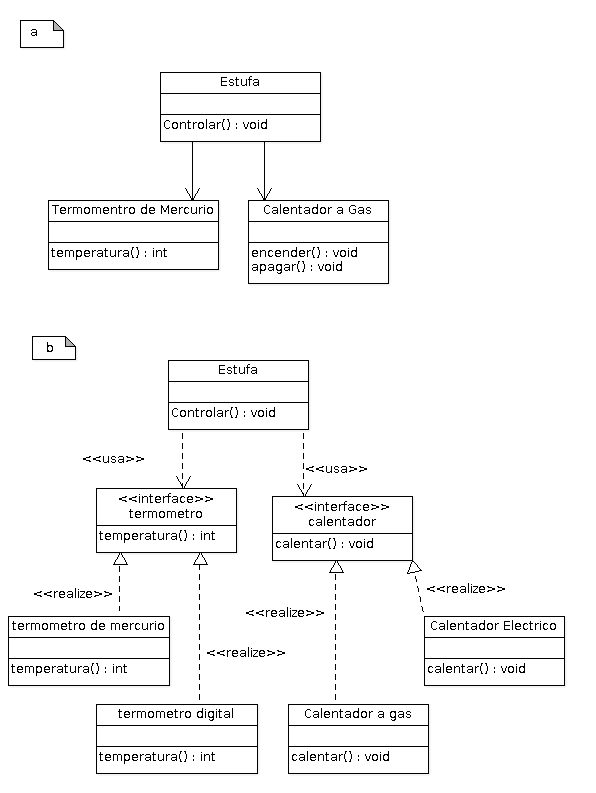
\includegraphics[scale=0.5]{./img/estufa.png} 

En \textit{a} vemos una estufa con su termómetro y su calentador de gas. En el código de calentar() de la estufa tendré algo así:
\begin{verbatim}
while (TRUE) {
    while ( termometro.temperatura() > MAX ) 	calentador.apagar()
    while ( termometro.temperatura() < MIN )	calentador.prender()
}
\end{verbatim} 

Si cambio el termómetro de mercurio por uno digital fui
esto es por que tengo el tipo de termómetro harcodeado en la estufa.
Una mejor solución seria lo que vemos en\textbf{ b}. Dependemos de abstracciones, 
si quiero cambio por el termómetro.

Mejor es depender de abstracciones. si, termómetro digital respeta
la interfaz toda la estufa debería andar sin problemas.
\\
\\
\textbf{ Nico-frases:}

\begin{itemize}
\item \textit{``Es más dueño de la interface quien la usa que quien la implenta''}
\item \textit{``Fool me once shame on you, fool me twice shame on me''}
que vendría a ser algo así como \textit{`` si me engañas una vez la culpa es tuya, si me engañas dos veces la culpa es mía ''} y viene a cuento de que si tengo hecho algo como la solución a de la estufa, es quizás por que nunca me dijeron que podría cambiar, pero el cliente ahora viene con el cambio, no puedo decirle haaa nunca me dijiste que podría cambiar..., entonces ya que estamos nos tomamos el trabajo de cambiar todo de modo que cuanto venga otro cambio, la estructura esté preparada para soportarlo.'' trantando de respetar lo mejor posibles los principios.

\end{itemize}




\subsection{LISKOV}
Los subtipos de una clase deben poder ``comportarse'' como el super tipo ó 
`` los subtipos de la clase tienen que poder reemplazar a los tipos de arriba sin que cambié
el comportamiento''


\subsubsection{Ejemplo: Rectángulo y cuadrado}
\begin{center}
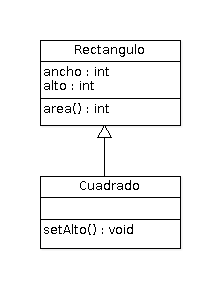
\includegraphics[scale=0.6]{./img/rectangulo-cuadrado.png} 
\end{center}

``Un Cuadrado, como un rectángulo, debe poder calcular su área''.
Un Cuadrado, ``es un'' rectángulo, el problema es que un cuadrado no se comporta igual que un 
rectángulo, en particular si tengo un setAlto(), en cuadrado, este también debe setear el ancho con el mismo número, bueno esto no vale en un rectángulo. No se están \textbf{comportando} igual.
la idea es la noción de ``es un'' en herencia tiene que ver con el comportamiento

\subsubsection{Ejemplo: Empleado mensual, por hora y voluntario.}
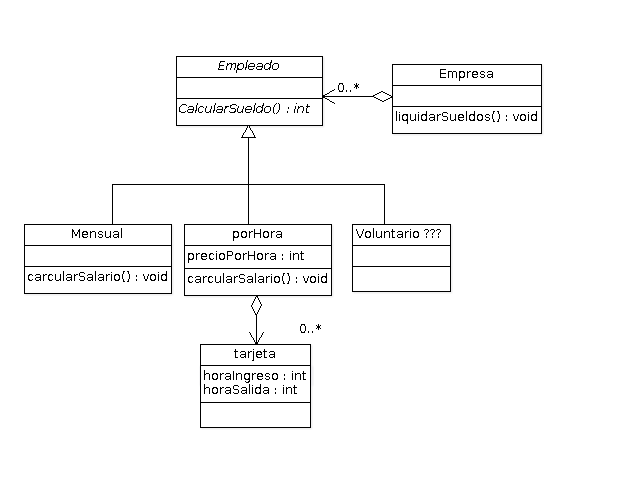
\includegraphics[scale=0.6]{./img/empleado-sueldo-voluntario.png}
 
El empleado mensual, por hora cobran un sueldo y el voluntario no cobra sueldo.
Pero el comportamiento que estoy capturando justamente es ese, el echo de cobrar sueldos.
El voluntario no se comporta como un empleado (en este caso).

Si no respeto LISKOV seguramente estoy rompiendo OCP
ya que para distinguir si es o no voluntario debo preguntar por el
tipo para darle un tratamiento especial. Dado que no se comporta como el tipo
base no puedo hacerlo genérico.

\subsection{ISP}
Las clases solo ven los métodos que usan.

\subsubsection{Ejemplo: Cajero automático.}
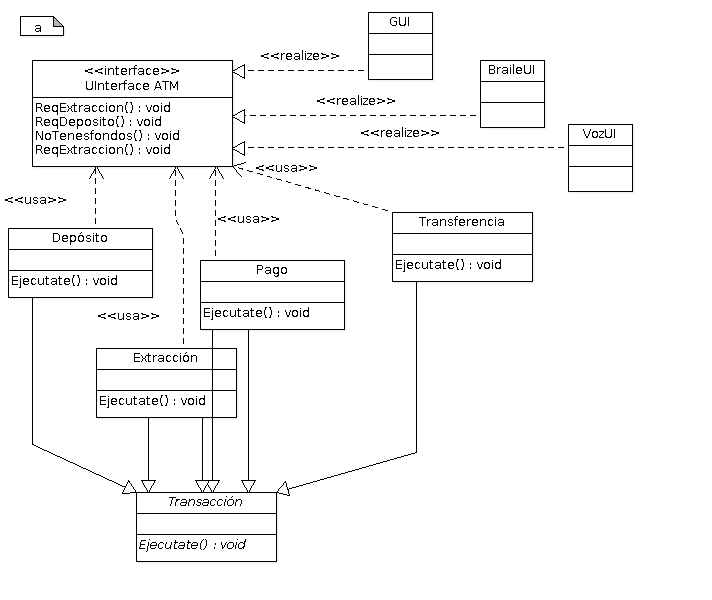
\includegraphics[scale=0.5]{./img/ATM-a.png} 
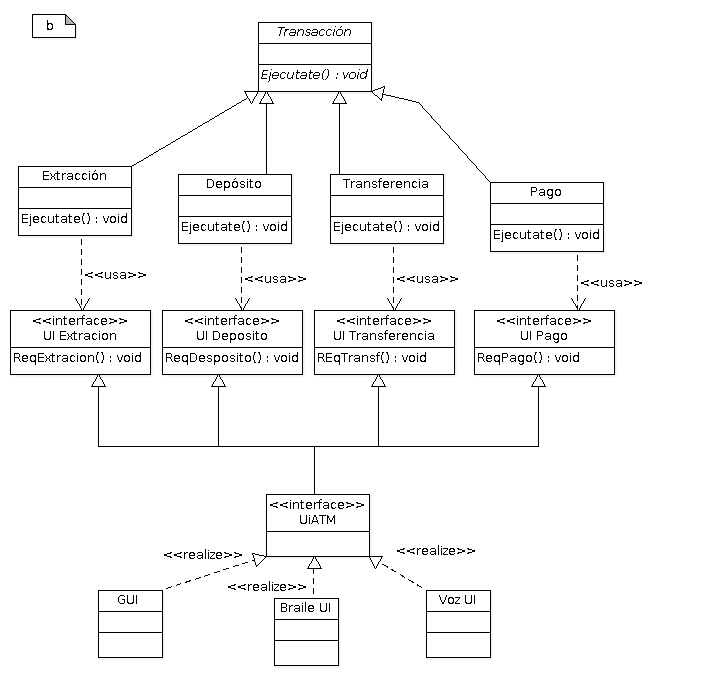
\includegraphics[scale=0.5]{./img/ATM-b.png} 
Vemos en \textbf{a} como la clase extracción por ejemplo tiene acceso a los métodos de deposito y transferencia, no hay una razón para ello. Esto es lo que se conoce como una interfaz demasiado gruesa, solución dividimos en una interfaz para cada funcionalidad, como en \textbf{b}.



\section{Resumen}

\begin{description}
\item[OCP:] (Open-Close Principle)
Tengo una clase a la que quiero agregarle funcionalidad, pero no quiero tocarla ya que
si la cambio debo re-testear todas las clases que la usan. Me baso en abstracciones.
Abierto para la extensión, cerrado para la modificación.

\item[SRP:] (Single Responsability Principle)
las clases deberían tener tienen una única razón ó eje de cambio.

\item[DIP:] (Dependency Inversion Principle)
Dependamos de cosas abstractas.

\item[LISKOV:] 
los hijos deberían poder comportarse como sus padres.

\item[ISP:] (Interface Segregation Principle)
Las clases solo ven los métodos que usan.

\end{description}




































\end{document}
